\documentclass[twocolumn,a4j]{jarticle}
\usepackage[dvipdfmx]{graphicx}

%%
%%
%% 以下のスタイル情報は変更しない
\setlength{\textheight}{277mm}
\setlength{\textwidth}{180mm}
\setlength{\topmargin}{-35mm}
\setlength{\oddsidemargin}{-9mm}

%%
%% 
%% 論文タイトルを記入
\title{
  感情表現に基づく人とロボットのインタラクションの設計
}

%%
%% 
%% 研究グループ、氏名、学籍番号、指導教員を記入
\author{
  佐賀大学 理工学部 理工学科 知能情報システム工学コース \\
   発表者:明石 華実(19238901) 指導教員:福田 修 教授,Yoeh Wen Liang プロジェクト助教
}



\begin{document}
\date{\empty}
\maketitle
\thispagestyle{empty}

\section{はじめに}
現在,世の中には様々な種類のペットロボットが存在している.これらには,飼い主との社会的交流の強いペットを目指しているものが多く,人間とのインタラクション設計は必要不可欠である.しかしながら,現在のペットロボットには,人間の多様な感情を汲み取り,インタラクションするものはなく,途中でユーザが飽きてしまうという致命的な問題がある\cite{ser2}\cite{ser1}.本研究は,感情表現に基づくインタラクションが,親密な関係構築に寄与するとの仮説に基づいている.このようなペットロボットを実現することで,お互いのインタラクションが親密になり,飽きの効果が軽減されることを期待する.提案技術により,一般家庭への普及や,医療福祉施設などへのアニマル・セラピーとしての普及がさらに進み,ペットロボットの必要性が向上すると考える.
% 現在、世の中には様々な種類のペットロボットが存在し,飼い主との社会的交流の強いペット(犬,猫等)を目指しているものが多い.しかしながら,現在のペットロボットには,人間の多様な感情を汲み取り,インタラクションするものがなく,途中でユーザが飽きてしまうという致命的な問題がある.本研究では,感情表現に基づくインタラクションが,親密な関係構築に寄与するとの仮説の証明を目指す.互いのインタラクションが増え,関係が親密になることで,飽きの効果軽減を期待する.

 %現在,世の中には様々な種類のペットロボットが存在する.これらには,飼い主との社会的交流の強いペット(犬,猫など)を目指しているものが多く,人間とのインタラクションの設計は必要不可欠である\cite{ser2}.しかしながら,途中でユーザが飽きてしまうという致命的な問題がある\cite{ser1}.
%\\人間と犬では,犬が飼い主の感情を汲み取り行動し,長い時間を共に過ごすことで,「情動の伝染」が起こると言われている\cite{ser3}.しかしながら,現在のペットロボットには,人間の多様な感情を汲み取り,インタラクションするものがない.本研究では,感情表現に基づくインタラクションが,親密な関係構築に寄与するとの仮説の証明を目指す.このようなペットロボットを実現することで,お互いのインタラクションが増え,関係が親密になることで,飽きの効果が軽減されることを期待する.提案技術により,一般家庭への普及や,医療福祉施設などへのアニマル・セラピーとしての普及が進み,ペットロボットの必要性は向上すると考える.
\vspace{-10mm}
\section{システム概要}

システムの概要を図1に示す.図に示すように人は自身の表情で感情を表現し,ペットロボットに伝える.ロボットはその表情をカメラ画像から認識し,認識結果に応じて行動する.このループにより,お互いの親密な関係を構築するのが狙いである.対象者はカメラ(Logicool C922n)に向かい感情を表現する.カメラから得られる動画像から,Amazon社のクラウドプラットフォーム,Amazon Web Services(以下AWS)を用いてリアルタイムに感情認識を行い,ワンボードマイコン(Rasberry Pi3 Model B)が,ペットロボットの関節に組み込まれたサーボモータ(Micro Servo 9g SG90)を制御する. 

\begin{figure}[h]
\begin{center}
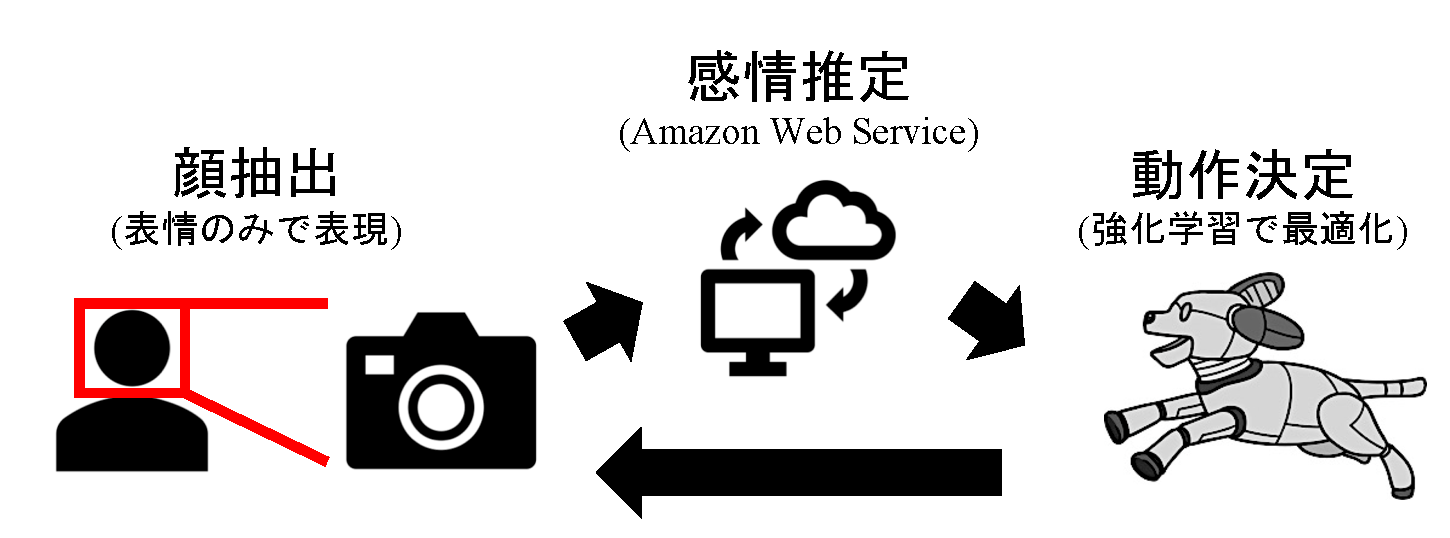
\includegraphics[scale=0.3]{System.eps}
\end{center}
\vspace{-5mm}
\caption{システム構成}
\label{System} %ここでは図のラベルを指定できます。詳しくはこの後記述します。
\end{figure}
%人 -> 感情表現 -> ロボット
%ロボット -> 反応(行動) -> 人
%の双方向の図が良いと思います.モータの部分はペットロボットが良いですね.
%表情の写真やロボットの写真を使うと図がカッコ良くなると思います.
\vspace{-10mm}
\section{感情表現推定の基礎実験}
 今回は,感情表現をインタラクションに使用可能であるかについて検証を行った.被験者は20代男性1名とし,指定される感情を5秒間,表情のみで表現する.指定される感情は, "HAPPY","CONFUSED","SURPRISED","FEAR","ANGRY","SAD","DISGUSTED","CALM"の8種類である.実験は各感情をランダムに指定することを1セットとし,3セット行った.
 実験の際の被験者へのフィードバックは,表\ref{Environment List}に示す4種類とした.
 %実験に用いる環境は4種類あり,「練習」,「見本」,「鏡」,「通常」とする.
 %「練習」とは,実験前に8種類の感情を任意の順番で表現してもらい,リアルタイムでフィードバックを行う環境である.「見本」とは,8種類の感情とそれに伴う一例が提示される環境である.「鏡」とは,実験時に被験者が自身の顔を確認できる環境である.「通常」とは,「練習」や「見本」,「鏡」がない環境である.

 \\実験は3種類で,フィードバックの条件は「なし」,「鏡\&見本」,「鏡\&見本\&認識結果」として順番で行った.
 被験者に指定した感情と,認識結果が一致した割合を, 正解率とする.感情認識結果の正解率を図\ref{Jikken}に示す.
 「鏡\&見本」では,「なし」と比べ平均正解率は15.0$%$上昇した.「鏡\&見本\&認識結果」をすることで,「なし」と比べてさらに平均正解率が58.3$%$と大幅に上昇した.「練習」により,高精度に感情認識が可能となり,インタラクションに利用できることが示された.

\vspace{-3mm}
\begin{table}[h]
\centering
\caption{フィードバック条件}
\begin{tabular}{|c|c|}
	\hline
		認識結果 & リアルタイムで結果をフィードバック \\
	\hline
		鏡 & 被験者が自身の顔を確認 \\
	\hline
		見本 & 8種類の典型的な表情が提示される \\
	\hline
		なし & フィードバックを行わない\\
	\hline
\end{tabular}
\label{Environment List}
\end{table}
\vspace{-5mm}

\begin{figure}[h]
\begin{center}
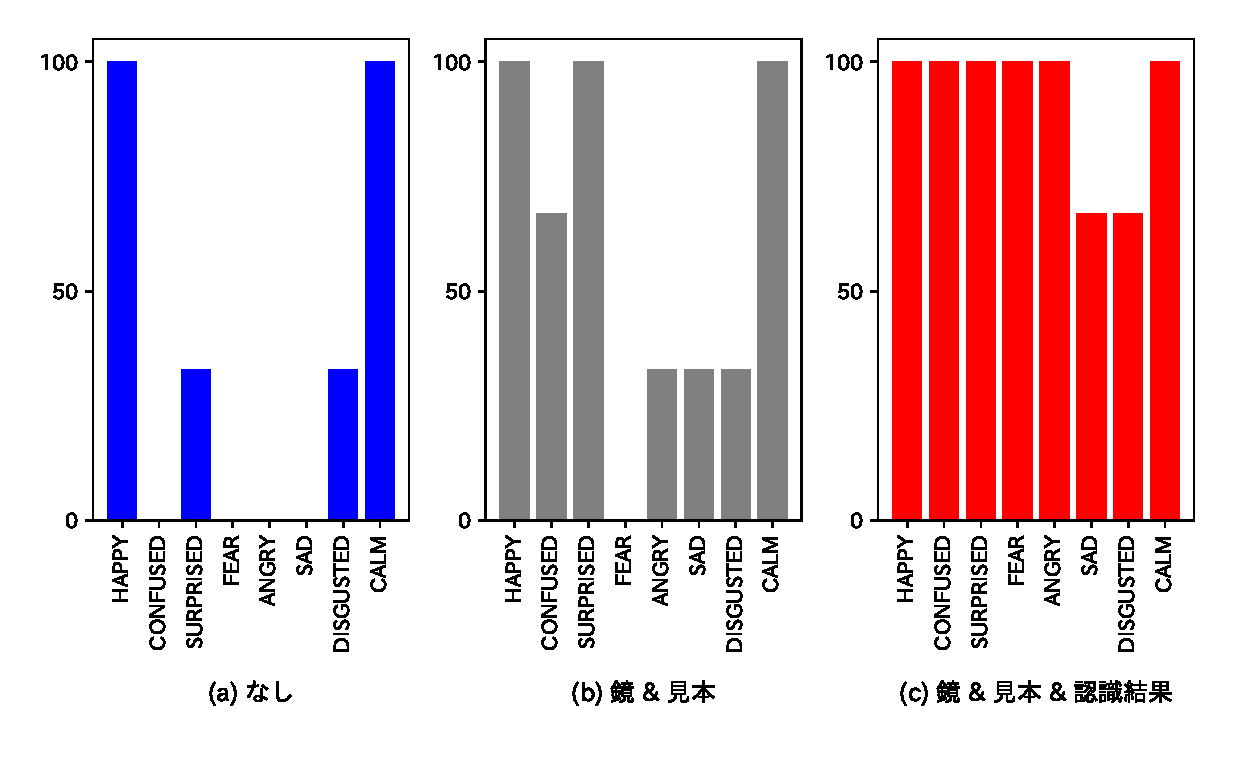
\includegraphics[scale=0.4]{Jikken.eps}
\end{center}
\vspace{-8mm}
\caption{実験結果}
\label{Jikken} %ここでは図のラベルを指定できます。詳しくはこの後記述します。
\end{figure}


\vspace{-10mm}
\section{まとめ}
本研究では,ペットロボットと人間とが,感情表現を用いたインタラクションを通して,飽きを軽減することを目指した.まず,表情のみで感情認識が可能か精度検証を行い,十分な精度を確認した.今後は,感情推定結果に基づき,行動するペットロボットの製作と効果の検証を目標とする.
%(サーボモータに制限せずに,推定結果に基づき行動するペットロボットの検討を行うとかでもいいのかなと思います.)
%また,制御されたサーボモータと触れ合うことで,インタラクションの増加,飽きの効果の軽減を検討する.



\vspace{-6mm}
\begin{thebibliography}{9}\setlength{\itemsep}{2ex}\small
\bibitem{ser2}
田中 一晶, 岡 夏樹, 躾による人間とペットロボットの関係の改善, 京都工芸繊維大学大学院工芸科学研究科, 第20回人工知能学会全国大会, 3F2-2, 4 pages, 2006.
\bibitem{ser1}
中田亨, ペット動物の対人心理作用能力のロボットにおける構築, 東京大学大学院工学系研究科, 学位論文, 2000.

%\bibitem{ser3}
%片山 真希, 心拍変動解析を用いたイヌ : ヒト間の不快情動伝染に関する研究 : Negative emotional contagion between dogs and humans using heart rate variability analysis, 麻布大学, http://id.nii.ac.jp/1112/00004521/,2017.

\end{thebibliography}
\end{document}

